\icode{E-MM-SI-L2-261011-002}
如图所示，牛顿摆是一组相互紧挨且悬挂在同一水平线上的相同小钢球，小明用牛顿摆进行探究活动。下列四组实验中左图为释放前的初始状态，右图为他预测的某些球升至最高点的状态，则下列选项中可能与实际情况相符的是\paren[]

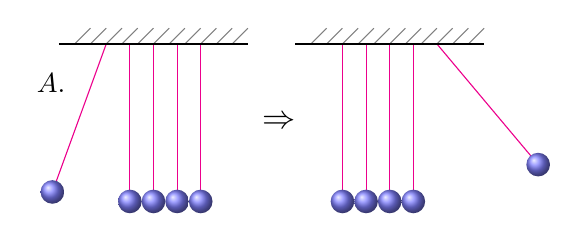
\begin{tikzpicture}
	\begin{scope}
		\draw[magenta] (0,0)--++(-110:2)coordinate(1);
		\shade[ball color=blue!50] (1) circle(.15);
		\foreach \x/\n in {.3/2,.6/3,.9/4,1.2/5}{
			\draw[magenta] (\x,0)--++(-90:2)coordinate(\n);
			\shade[ball color=blue!50] (\n) circle(.15);}
		\foreach \x in {-.4,-.2,...,1.6}
			\draw[gray] (\x,0)--++(.2,.2);
		\draw[thick] (-.6,0)--(1.8,0);
	\end{scope}
	\begin{scope}[xshift=3cm]
		\draw[magenta] (1.2,0)--++(-50:2)coordinate(5);
		\shade[ball color=blue!50] (5) circle(.15);
		\foreach \x/\n in {0/1,.3/2,.6/3,.9/4}{
			\draw[magenta] (\x,0)--++(-90:2)coordinate(\n);
			\shade[ball color=blue!50] (\n) circle(.15);}
		\foreach \x in {-.4,-.2,...,1.6}
			\draw[gray] (\x,0)--++(.2,.2);
		\draw[thick] (-.6,0)--(1.8,0);
	\end{scope}
	\node at(2.2,-1){\large\(\Rightarrow\)};
	\node at(-.7,-.5){\(A.\)};
\end{tikzpicture}
\hspace{2em}
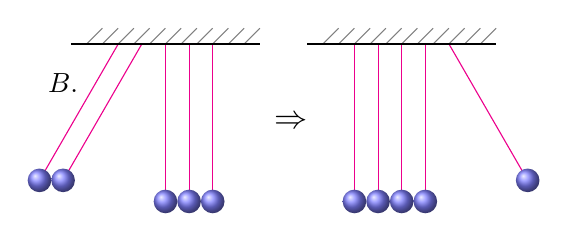
\begin{tikzpicture}
	\begin{scope}
		\foreach \x/\n in {0/1,.3/2}{
			\draw[magenta] (\x,0)--++(-120:2)coordinate(\n);
			\shade[ball color=blue!50] (\n) circle(.15);}
		\foreach \x/\n in {.6/3,.9/4,1.2/5}{
			\draw[magenta] (\x,0)--++(-90:2)coordinate(\n);
			\shade[ball color=blue!50] (\n) circle(.15);}
		\foreach \x in {-.4,-.2,...,1.6}
			\draw[gray] (\x,0)--++(.2,.2);
		\draw[thick] (-.6,0)--(1.8,0);
	\end{scope}
	\begin{scope}[xshift=3cm]
		\draw[magenta] (1.2,0)--++(-60:2)coordinate(5);
		\shade[ball color=blue!50] (5) circle(.15);
		\foreach \x/\n in {0/1,.3/2,.6/3,.9/4}{
			\draw[magenta] (\x,0)--++(-90:2)coordinate(\n);
			\shade[ball color=blue!50] (\n) circle(.15);}
		\foreach \x in {-.4,-.2,...,1.6}
			\draw[gray] (\x,0)--++(.2,.2);
		\draw[thick] (-.6,0)--(1.8,0);
	\end{scope}
	\node at(2.2,-1){\large\(\Rightarrow\)};
	\node at(-.7,-.5){\(B.\)};
\end{tikzpicture}

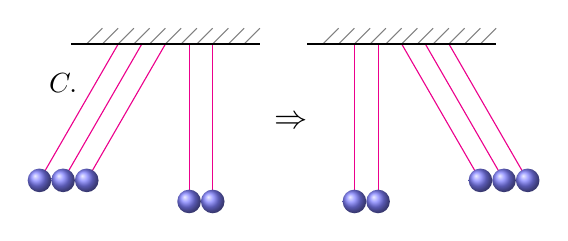
\begin{tikzpicture}
	\begin{scope}
		\foreach \x/\n in {0/1,.3/2,.6/3}{
			\draw[magenta] (\x,0)--++(-120:2)coordinate(\n);
			\shade[ball color=blue!50] (\n) circle(.15);}
		\foreach \x/\n in {.9/4,1.2/5}{
			\draw[magenta] (\x,0)--++(-90:2)coordinate(\n);
			\shade[ball color=blue!50] (\n) circle(.15);}
		\foreach \x in {-.4,-.2,...,1.6}
			\draw[gray] (\x,0)--++(.2,.2);
		\draw[thick] (-.6,0)--(1.8,0);
	\end{scope}
	\begin{scope}[xshift=3cm]
		\foreach \x/\n in {.6/3,.9/4,1.2/6}{
			\draw[magenta] (\x,0)--++(-60:2)coordinate(\n);
			\shade[ball color=blue!50] (\n) circle(.15);}
		\foreach \x/\n in {0/1,.3/2}{
			\draw[magenta] (\x,0)--++(-90:2)coordinate(\n);
			\shade[ball color=blue!50] (\n) circle(.15);}
		\foreach \x in {-.4,-.2,...,1.6}
			\draw[gray] (\x,0)--++(.2,.2);
		\draw[thick] (-.6,0)--(1.8,0);
	\end{scope}
	\node at(2.2,-1){\large\(\Rightarrow\)};
	\node at(-.7,-.5){\(C.\)};
\end{tikzpicture}
\hspace{2em}
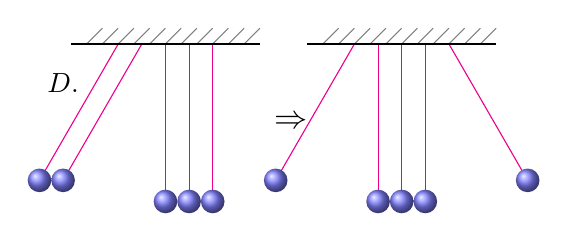
\begin{tikzpicture}
	\begin{scope}
		\foreach \x/\n in {0/1,.3/2}{
			\draw[magenta] (\x,0)--++(-120:2)coordinate(\n);
			\shade[ball color=blue!50] (\n) circle(.15);}
		\foreach \x/\n in {.6/3,.9/4,1.2/5}{
			\draw[magenta] (\x,0)--++(-90:2)coordinate(\n);
			\shade[ball color=blue!50] (\n) circle(.15);}
		\foreach \x in {-.4,-.2,...,1.6}
			\draw[gray] (\x,0)--++(.2,.2);
		\draw[thick] (-.6,0)--(1.8,0);
	\end{scope}
	\begin{scope}[xshift=3cm]
		\foreach \x/\n in {1.2/5}{
			\draw[magenta] (\x,0)--++(-60:2)coordinate(\n);
			\shade[ball color=blue!50] (\n) circle(.15);}
		\foreach \x/\n in {0/1}{
			\draw[magenta] (\x,0)--++(-120:2)coordinate(\n);
			\shade[ball color=blue!50] (\n) circle(.15);}
		\foreach \x/\n in {.3/2,.6/3,.9/4}{
			\draw[magenta] (\x,0)--++(-90:2)coordinate(\n);
			\shade[ball color=blue!50] (\n) circle(.15);}
		\foreach \x in {-.4,-.2,...,1.6}
			\draw[gray] (\x,0)--++(.2,.2);
		\draw[thick] (-.6,0)--(1.8,0);
	\end{scope}
	\node at(2.2,-1){\large\(\Rightarrow\)};
	\node at(-.7,-.5){\(D.\)};
\end{tikzpicture}
\begin{answer}
    C\qquad 提示：弹性碰撞质量相等，交换速度
\end{answer}